% This is the Reed College LaTeX thesis template. Most of the work
% for the document class was done by Sam Noble (SN), as well as this
% template. Later comments etc. by Ben Salzberg (BTS). Additional
% restructuring and APA support by Jess Youngberg (JY).
% Your comments and suggestions are more than welcome; please email
% them to cus@reed.edu
%
% See http://web.reed.edu/cis/help/latex.html for help. There are a
% great bunch of help pages there, with notes on
% getting started, bibtex, etc. Go there and read it if you're not
% already familiar with LaTeX.
%
% Any line that starts with a percent symbol is a comment.
% They won't show up in the document, and are useful for notes
% to yourself and explaining commands.
% Commenting also removes a line from the document;
% very handy for troubleshooting problems. -BTS

% As far as I know, this follows the requirements laid out in
% the 2002-2003 Senior Handbook. Ask a librarian to check the
% document before binding. -SN

%%
%% Preamble
%%
% \documentclass{<something>} must begin each LaTeX document
\documentclass[12pt,twoside]{reedthesis}
% Packages are extensions to the basic LaTeX functions. Whatever you
% want to typeset, there is probably a package out there for it.
% Chemistry (chemtex), screenplays, you name it.
% Check out CTAN to see: http://www.ctan.org/
%%
\usepackage{graphicx,latexsym}
\usepackage{amssymb,amsthm,amsmath}
\usepackage{longtable,booktabs,setspace}
\usepackage{chemarr} %% Useful for one reaction arrow, useless if you're not a chem major
\usepackage[hyphens]{url}
\usepackage[page]{appendix}
\usepackage{rotating}
\usepackage{natbib}
\usepackage{pgfplots}
\usepackage{color}
\usepackage{xcolor}
\usepackage{listings}
\usepackage{caption}
% A better code font
\usepackage{inconsolata}
\lstset{
    language=C,
    keywordstyle=\color{blue},
    basicstyle=\footnotesize\ttfamily,
    commentstyle=\color{gray}
}

\DeclareCaptionFont{white}{ \color{white} }
\DeclareCaptionFormat{listing}{
  \colorbox[cmyk]{0.43, 0.35, 0.35,0.01 }{
    \parbox{\textwidth}{\hspace{15pt}#1#2#3}
  }
}
\captionsetup[lstlisting]{ format=listing, labelfont=white, textfont=white, singlelinecheck=false, margin=0pt }

\lstdefinelanguage
   [x64]{Assembler}     % add a "x64" dialect of Assembler
   [x86masm]{Assembler} % based on the "x86masm" dialect
   % with these extra keywords:
   {morekeywords={CDQE,CQO,CMPSQ,CMPXCHG16B,JRCXZ,LODSQ,MOVSXD, %
                  POPFQ,PUSHFQ,SCASQ,STOSQ,IRETQ,RDTSCP,SWAPGS, %
                  MOVAPD,SUBPD,MULSD,SHUFPD,ADDSD,XORPS,SQRTSD, %
                  MOVDDUP,DIVSD,DIVPD,MULPD,ADDPD %
                  rax,rdx,rcx,rbx,rsi,rdi,rsp,rbp, %
                  r8,r8d,r8w,r8b,r9,r9d,r9w,r9b, %
                  r10,r10d,r10w,r10b,r11,r11d,r11w,r11b, %
                  r12,r12d,r12w,r12b,r13,r13d,r13w,r13b, %
                  r14,r14d,r14w,r14b,r15,r15d,r15w,r15b}} % etc.


\pgfplotsset{compat=1.5}
\usepackage[alsoload=astro]{siunitx}
% Comment out the natbib line above and uncomment the following two lines to use the new
% biblatex-chicago style, for Chicago A. Also make some changes at the end where the
% bibliography is included.
%\usepackage{biblatex-chicago}
%\bibliography{thesis}


\usepackage{fbb} % other fonts are available like times, bookman, charter, palatino

\title{N-Body Simulations of Barred Galaxies}
\author{Thomas B Malthouse}
% The month and year that you submit your FINAL draft TO THE LIBRARY (May or December)
\date{Summer 2017}
\division{Mathematics and Natural Sciences}
\advisor{J Powell}
%If you have two advisors for some reason, you can use the following
%\altadvisor{Your Other Advisor}
%%% Remember to use the correct department!
\department{Physics}


\setlength{\parskip}{1.5em}

\DeclareSIUnit[]\solar
{\mathrm{\ensuremath{M}}_\odot}
\DeclareSIUnit[]\year
{\mathrm{\ensuremath{yr}}}

\definecolor{light-gray}{gray}{0.9}
\newcommand\code[1]{\colorbox{light-gray}{\texttt{\textcolor{black}{#1}}}}


%%
%% End Preamble
%%
%% The fun begins:
\begin{document}

  \maketitle
  \frontmatter % this stuff will be roman-numbered
  \pagestyle{empty} % this removes page numbers from the frontmatter

% Acknowledgements (Acceptable American spelling) are optional
% So are Acknowledgments (proper English spelling)
    \chapter*{Acknowledgements}
	I want to thank a few people.

% The preface is optional
% To remove it, comment it out or delete it.
    \chapter*{Preface}
	This is an example of a thesis setup to use the reed thesis document class.



    \chapter*{List of Abbreviations}
		You can always change the way your abbreviations are formatted. Play around with it yourself, use tables, or come to CUS if you'd like to change the way it looks. You can also completely remove this chapter if you have no need for a list of abbreviations. Here is an example of what this could look like:

	\begin{table}[h]
	\centering % You could remove this to move table to the left
	\begin{tabular}{ll}
		\textbf{ABC}  	&  American Broadcasting Company \\
		\textbf{CBS}  	&  Columbia Broadcasting System\\
		\textbf{CDC}  	&  Center for Disease Control \\
		\textbf{CIA}  	&  Central Intelligence Agency\\
		\textbf{CLBR} 	&  Center for Life Beyond Reed\\
		\textbf{CUS}  	&  Computer User Services\\
		\textbf{FBI}  	&  Federal Bureau of Investigation\\
		\textbf{NBC}  	&  National Broadcasting Corporation\\
	\end{tabular}
	\end{table}


    \tableofcontents
% if you want a list of tables, optional
    \listoftables
% if you want a list of figures, also optional
    \listoffigures

% The abstract is not required if you're writing a creative thesis (but aren't they all?)
% If your abstract is longer than a page, there may be a formatting issue.
    \chapter*{Abstract}
	The preface pretty much says it all.

	\chapter*{Dedication}
	You can have a dedication here if you wish.

  \mainmatter % here the regular arabic numbering starts
  \pagestyle{fancyplain} % turns page numbering back on

%The \introduction command is provided as a convenience.
%if you want special chapter formatting, you'll probably want to avoid using it altogether

    \chapter*{Introduction}
         \addcontentsline{toc}{chapter}{Introduction}
	\chaptermark{Introduction}
	\markboth{Introduction}{Introduction}
	% The three lines above are to make sure that the headers are right, that the intro gets included in the table of contents, and that it doesn't get numbered 1 so that chapter one is 1.

% Double spacing: if you want to double space, or one and a half
% space, uncomment one of the following lines. You can go back to
% single spacing with the \singlespacing command.
% \onehalfspacing
% \doublespacing

The Milky Way is an entirely unextraordinary galaxy. Its hallmark spiral arms---visible in the night sky as a bright smearing of stars, stretching from horizon to horizon---are shared by about 60\% of galaxies in our universe \citep{apm-bgc}. A bar---a large collection of stars passing through the galactic center, prominent in renderings of the Milky Way (such as Fig. \ref{ssc2008})---is also found around two in three other spiral galaxies. Under the Hubble classification system commonly used to sort and organize galaxies, the Milky Way is classified as an \emph{Sb} type galaxy, along with 40\% of known galaxies (for more information, see \ref{hubble-fork}). These extensive similarities mean that studying the evolution and structure of the Milky Way can provide insights about galactic behavior in general, and that observing other galaxies can reveal the past and future of out own.

\begin{figure}[p]
    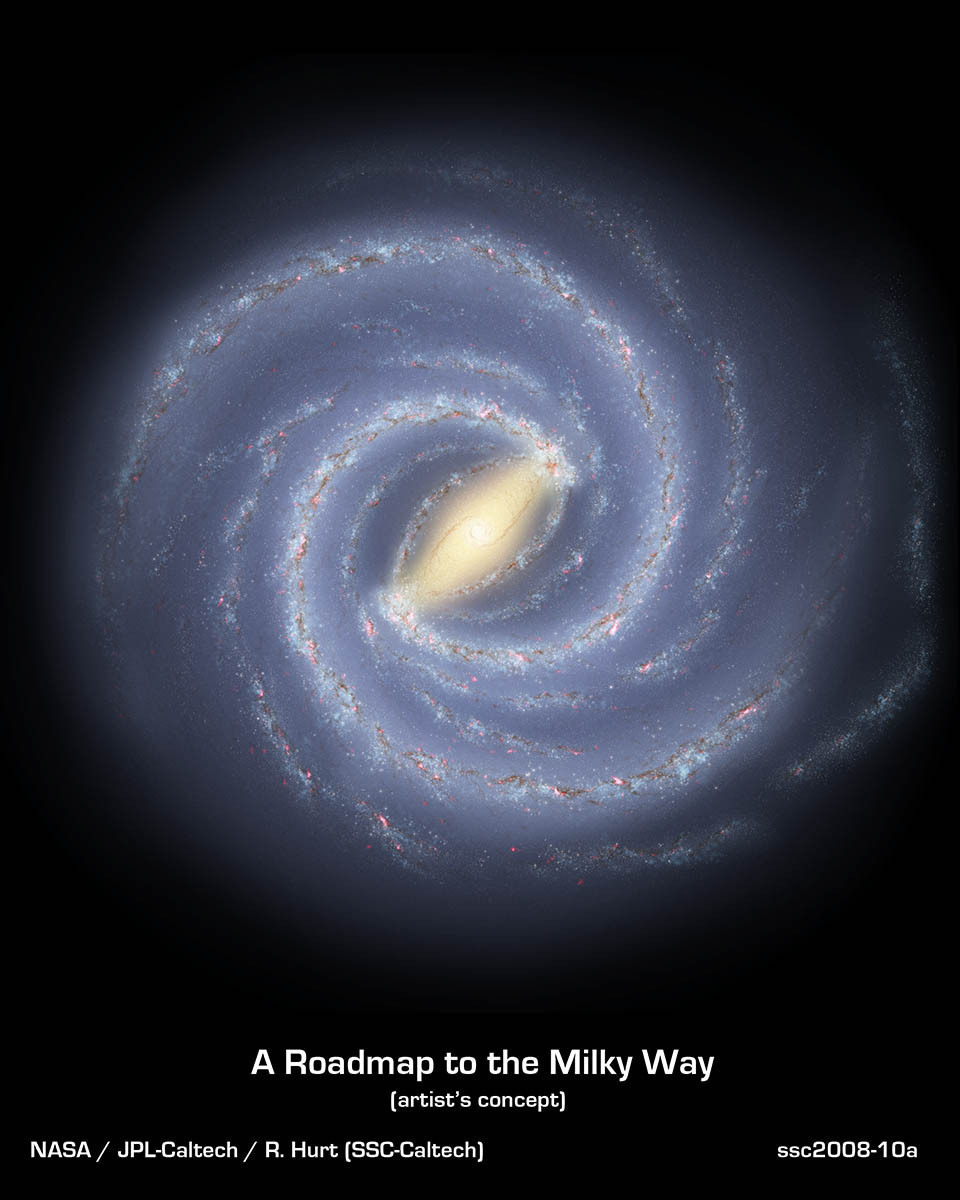
\includegraphics[width=\textwidth,height=\textheight,keepaspectratio]{imgs/ssc2008-10a_Sm}
    \caption{This rendering of the Milky Way clearly shows the stellar bar going through the center of the galaxy, and the extensive spiral system. \emph{Image courtesy NASA/JPL}}
    \label{ssc2008}
\end{figure}

\section*{Disks}
The Milky Way has two main disks which hold the vast majority of visible matter in the galaxy and give rise to its spiral structure. The \emph{thin disk} is the more visible of the two, composed mainly of main-sequence stars and clouds of gas and dust \citep{galaxies-in-universe}. Its vertical density scale height---the distance over which its density decreases by a factor of $e$---is about $\SI{350}{\parsec}$---very thin compared to its radius of about $\SI{25}{\kilo\parsec}$. This thinness comes from its young age, since the stars that compose it are less likely to have had their orbits perturbed---especially in the chaotic period about $\SI{9}{\giga\year}$ ago. The thin disk accounts for about 97\% of the galaxy's (normal) mass and holds nearly all galactic dynamism and stellar formation.

The other disk, referred to as the \emph{dark disk} or \emph{thick disk}, is far older and less dynamic \citep{starrfield-thick-disk}. Composed of stars formed $\SI{10}{\giga\year}$ to $\SI{12}{\giga\year}$ ago, it is very faint and hard to detect---all the bright stars burned out long ago, and the only ones left are low-magnitude red dwarfs and K-class stars. These stars' orbits also tend to be less regular, since they've had time to be perturbed and pushed into new orbits, especially during the chaotic initial organization of the Milky Way $\SI{10}{\giga\year}$ ago---resulting in a scale height of about $\SI{1}{\kilo\parsec}$. Because its stars are so steady-burning and the complete lack of gas and dust, the thick disk is very stable and exhibits none of the dynamism seen in the thin disk. It accounts for only about 3\% of the regular matter in the galaxy, with a total mass of about $\SI{1e10}{\solar}$.
Note that the name \emph{dark disk} refers to the low luminosity of the stars within, and has no relation to the dark matter discussed below.

\section*{Metallicity and Age}
The easiest way to determine which disk a star is in is to look at its metallicity (the amount of metal in the star.) This can be measured by looking at the strength of various emission spectra, since elements like iron have very distinct emission lines. These heavy elements are only formed when large stars reach the end of their life, and so their concentration has steadily increased over time as more large stars form and die. Old stars dating back to the formation of the galaxy (like those of the thick disk) tend to have very ``clean'' emission spectra, with very little other than hydrogen and helium, while younger stars have strong magnesium and iron lines.

Metallicity isn't a perfect way to measure the age of a star. Metal concentrations vary widely across both space and time, and two stars forming at the same time may have very different metallicities. However, when looking at a large and statistically representative sample of stars, a high metallicity indicates a younger age \citep[pp. 885]{modern-astrophysics}.

\section*{The Stellar Halo}

The disks extend to about $\SI{25}{\kilo\parsec}$ from the galactic center, and contain practically all the mass within that radius. Past that point, however, stars are distributed far more chaotically. The thin plane disappears, and stellar orbits become more spherically distributed. The composition of individual stars in the halo is similar to those in the thick disk---old, dim, and unchanging. However, the halo is also home to many globular clusters, groups of tens or hundreds of thousands of stars that act like small galaxies in their own right. These clusters continue to create new stars, and most of the light coming from the halo is from globular clusters.

Measurements of stellar velocities have long predicted that the mass of the halo dominates the mass of the galaxy---about 95\% of galactic mass must be in the halo for the observed velocity curves to hold. Since the halo was known not to be made up of gas and dust (otherwise its extinctive properties would be easy to measure), astronomers long though that the halo contained vast numbers of dense, dark bodies, such as lone planets, dim stars, black holes, and neutron stars---referred to as MACHOs, or Massive Astrophysical Compact Halo Object. Gravitational lensing observations disproved this theory, however, when they capped the mass percentage of MACHOs at about 15\% of the mass of the galaxy. The remainder of the mass was some strange material, spherically distributed throughout the universe, that interacts with nothing but gravity.

\section*{Dark Matter}
As that strange material was further studied (as much as it is possible to study something so elusive), more of its properties were discovered. This \emph{dark matter} seems to be made up of WIMPS (Weakly Interacting Massive Particles), which only interact via gravity and the weak force. Being collisionless (since it does not interact with the electromagnetic force), it does not coalesce and form clouds and stars like regular matter, which is how it has maintained its spherical distribution for so long.

This dark matter has a density of
\begin{equation}
    \rho(r) = \frac{\rho_0}{\left(\frac{r}{a}\right)\left(1+\frac{r}{a}\right)^2}
\end{equation}
where $\rho_0$ is the maximum density and $a$ is proportional to the size of the galaxy. This function is referred to as the NFW profile (named after its creators, Navarro, Frank, and White), and is highly accurate for all observed spiral galaxies. For the Milky Way, the simplified equation
\begin{equation}
    \rho(r) = \frac{\rho_0}{1+\left(\frac{r}{1}\right)^2}
\end{equation}
also returns satisfactory results. However, both these equations appear to suffer from a major problem. If we use them to calculate the total mass of the dark matter in a galaxy, integrating from 0 to $\infty$, it appears that a galaxy has an infinite mass, as follows:
\begin{equation}
    \int\limits_{0}^{\infty} \rho(r) 4 \pi r^2 \, \text{d}r = \infty
\end{equation}
Since we know this is not true, there must be a cutoff point where the law no longer holds. As it turns out, in local groups like our own, the dark matter halos are so large that they border one another---providing a natural cutoff point and a solution to our problem \citep[pp. 196]{galaxies-in-universe}.

\section*{Coordinate Systems}

To identify and keep track of objects in the sky, we need to create a coordinate system. A number of natural possibilities spring to mind. The three most useful are detailed below.

\subsection*{Equatorial Coordinates}

An equatorial coordinate has two components---a \emph{right ascension}, and a \emph{declination}. To find this coordinate, find the location on the Earth's surface where the object of interest is directly overhead, in the very middle of the sky. The right ascension is the angle between the nearest point on the equator and the vernal equinox (which is defined to be the point where the equator crosses the ecliptic). The declination is then the angle between the current point and that nearest equatorial point. This coordinate system is very ancient, dating back millennia. Figure \ref{equatorial-coords} shows the process of finding such a coordinate.

\begin{figure}[p]
    \includegraphics{imgs/equat.png}
    \caption{This figure shows the process of finding an equatorial coordinate. CNP and CSP refer to the celestial north and south poles, respectively. R. Ascension refers to the right ascending node, where the Earth's rotational plane crosses its orbital plane.}
    \label{equatorial-coords}
\end{figure}

\subsection*{Galactic Coordinates}

This coordinate system is similar to the equatorial system, but the declination is measured from the galactic plane instead of the equatorial plane. The right ascension is then defined to be the angle between the projection of the body of interest on the galactic plane and the vector between the Sun and galactic center. Figure \ref{galactic-coords} shows this process in more detail. Although harder to calculate from the surface of the earth, this system is more natural when studying bodies traveling close to the Sun. The standard notation and conversions between the two systems are given below:

\begin{tabular}{lll} \toprule
    Measurement & Equatorial Notation & Galactic Notation \\ \midrule
    Right Ascension &  $\delta$       & $b$               \\
    Declination     &  $\alpha$       & $\ell$            \\ \bottomrule
\end{tabular}

\begin{equation}
    \sin b = \sin \delta_{NGP} \sin \delta + \cos \delta_{NGP} \cos \delta \cos (\alpha-\alpha_{NGP})
\end{equation}
\begin{equation}
    \sin \delta = \sin \delta_{NGP} \sin b + \cos \delta_{NGP} \cos b \cos{\ell_{NCP} - \ell}
\end{equation}
Where $\delta_{NGP} = \ang{27;7;41.7}$ and $\ell_{NCP}=\ang{123;55;55.2}$, as determined by the tilt of the earth and its orientation relative to the galactic plane. These equations can also be inverted to find $\ell$ and $\alpha$ \citep[pp. 900]{modern-astrophysics}.

\begin{figure}[p]
    \includegraphics{imgs/galactic}
    \caption{This figure shows the process of finding a galactic coordinate. GNP and GSP refer to the galactic north and south poles, respectively.}
    \label{galactic-coords}
\end{figure}

\subsection*{Cylindrical Coordinates}

The two coordinate systems discussed earlier are well-suited for positional observations from the Earth at a given point in time, but perform poorly over long timeframes. As the sun travels around its orbit, the coordinates of an object change even if it has not moved at all---not an ideal behavior from a reference system. The cylindrical coordinate system, with a reference point at the center of the universe solves these concerns. Unlike the others, it is a three-component coordinate system: $R$ is the radial distance along the plane, increasing outwards; $\theta$ is the angular position, and increases in the direction of rotation; and $z$ is the height above (or below) the plane, increasing towards the north, as shown in figure \ref{cylindrical-coords}. These coordinates also produce a natural (and commonly used) velocity coordinate system, as described below \citep{modern-astrophysics}:
\begin{equation}
    \Pi \equiv \frac{dR}{dt} \hspace{2cm} \Theta \equiv R\frac{d\theta}{dt} \hspace{2cm} Z \equiv \frac{dz}{dt}
\end{equation}

Note that, because the galaxy rotates clockwise when viewed from the north pole, this is a left-handed coordinate system rather than a more-standard right-hand system. Fortunately, we do not need to take any cross-products, so this does not cause any problems.

\begin{figure}[p]
    \includegraphics{imgs/cyl-coords}
    \caption{This figures shows the process of finding a cylindrical coordinate.}
    \label{cylindrical-coords}
\end{figure}

\subsection*{Local Standard of Rest}

Now that we have a definition of the cylindrical velocity coordinates, we can define the Local Standard of Rest (LSR), an important concept in astrophysics. The LSR at a given moment is defined to be the velocity of a body in the sun's position, in a perfectly circular and on-plane orbit---which in practice means the $\Theta$-component of the sun's velocity, with $\Pi$ and $Z$ set to zero.

The velocity of a nearby star relative to the LSR is known as its \emph{peculiar velocity}, and approximates the velocity of that star relative to the sun. Its coordinates are typically designated $(u,v,w)$, where
\begin{align}
    u &= \Pi - \Pi_{LSR} \\
    v &= \Theta - \Theta_{LSR} \\
    w &= Z - Z_{LSR}
\end{align}

The average peculiar velocity for stars in the solar neighborhood is approximately zero, since the universe is mostly axisymmetric. However, individual peculiar velocities vary widely, with young main-sequence stars like the sun having low velocities and old, metal-poor red dwarfs having higher velocities. As discussed earlier, this is due to the additional orbital perturbations experienced by old stars, especially during the chaotic period of formation $\SI{9}{\giga\year}$ ago.

\chapter{Computational Optimizations}

[[I am really glad to see this section start to develop, but when you get a chance to add a bunch of meta-discourse/introduction that would be great.  Why C instead of C++ -- type of discussion. Where learn C -- ``... the hard way.''  Some overall  comments on programming and hardware for N-body simulations.  Vectors are clearly very cool, but it seems a bit deep for a start. Indicate level of computer science education that you are writing for and give your old texts are refs. For example, compiler definition.  ]]

Simulating a galaxy requires a massive amount of computational power. Even a simple statistical approximation, with a couple hundred or thousand bodies, involves hundreds of thousands of calculations every timestep. Multiplied by 30 updates per second (to ensure smooth graphics), we quickly become responsible for hundreds of millions of calculations every second. To achieve that kind of performance, we need to understand how modern computer hardware functions and how various programming languages take advantage of that.

\subsection{Assembly and Machine Code}
Every computer program ever written can be expressed rewritten with a small set of commands. These commands directly manipulate memory, adding, comparing, and copying bits around. Different types of computer processors have different sets of commands, some more extensive than others. For example, the ARM processors found in smartphones have a \emph{RISC} (reduced instruction set circuit) design, which means they can perform a minimal set of operations, and more complex operations---like the square root---are expressed in terms of that small set. Other architectures, like the x86 design found in nearly all modern laptops and desktops, are referred to as \emph{CISC} (complex instruction set circuit) designs, and can do more operations without being programmed to. This design is often faster, but is more difficult to manufacture and often more expensive. In this thesis, we will exclusively focus on the x86\_64 architecture, as found in nearly all modern desktop and laptop computers.

The set of operations a processor can perform is referred to as the \emph{instruction set}, and is determined entirely by the physical circuit of the processor---so an x86 processor can never be turned into an ARM processor, or vice versa. As the processor runs, instructions are provided in the form of 8-bit numbers, each one corresponding to an operation. For example, the \emph{opcode} \code{0x40} (decimal 64) tells the processor to increment a given value by one. Since the processor also needs to know what data to perform the operation on, a more complete instruction would look something like \code{0x40 6c}. This instruction increments the value stored in memory at location \texttt{6c} by one.

Early programs were written like this, as long sequences of hexadecimal numbers that could be directly interpreted by the processor. However, remembering dozens of opcodes was unwieldy, and finding and fixing bugs was practically impossible. Frustrated, programmers invented human-friendly names for operations and common memory locations and wrote a tool (called an \emph{assembler}) to automatically replace them with the appropriate number. This new programming language was called \emph{assembly}, and greatly simplified programming. For example, our instruction from earlier would be written in assembly as something like \code{INC EAX}---still opaque, but more useful than a few hexadecimal numbers. Many programs still in use today (including Unix, the basis of Mac OS X and Linux) were originally written in an assembly language.

\subsection{The Development of High-level Languages}

Assembly was a massive improvement over typing in raw machine code, but it remained difficult to write and maintain large codebases, especially with large teams of programmers. Simple tools like conditional (if/else) blocks and loops were error-prone, and the structure of the program mimicked the inner working of the processor more than that of the human brain. Various \emph{programming languages} were designed to simplify the programming process, with associated \emph{compilers} to convert source code into assembly. These languages featured more natural math and now-familiar constructs like the \code{for} loop and the concept of functions. The most popular and enduring of these languages was C, which underlies nearly every operating system and utility in use today. Our example instruction from earlier, written in C, is \code{i++;}---far simpler than before, and close to the notation used in mathematics.

Of course (and this should seem familiar by this point), C had some limitations. String handling was an exercise in frustration, and manually handling memory meant leaks (where a piece of memory is never returned to the operating system) were commonplace. Accessing invalid memory was all-too-common, especially among new programmers, and could lead to all kinds of insidious bugs. Higher-level languages were created to deal with these problems, providing robust, error-free constructs to simplify these tasks. The first and most well-known of these languages was C++, which started out as a collection of text replacements and code generators for C and quickly evolved into a massive, full-featured language. Others followed, many keeping the basic syntax of C but automating ever-more. In general, these languages were much easier to write than C, at a significant performance cost---which was offset by rapid improvements in processor technology.

\subsection{Choosing a Language}
As mentioned earlier, performance is absolutely critical for our n-body simulator. Therefore, we need to be very careful when choosing a programming language for our project. Modern \emph{Interpreted languages}---which do not compile to machine code, but are run by an \emph{interpreter} or \emph{virtual machine}---like Python or C\# have too much overhead to use. Their simplicity and ease of use would be very nice to have, but they just aren't fast enough for our purposes. That leaves us with the compiled languages---C and C++ the most well known among them.

At first, C++ would seem like an obvious choice. Features like exceptions (which greatly improve error handling) and inheritance (which makes it easier to work with complex data types) are hard to live without, and most programmers have never used a language without them. However, these features also add overhead---they function as code generators, making it easy to create a lengthy and computationally complex program without realizing it. Since we can't use most of the features that make C++ what it is for performance reasons, the choice between C and C++ is mostly cosmetic---the finished codes would look very similar, and could easily be converted into each other. Since I had more experience with C from prior project and much prefer the C syntax to that of C++, I decided to use C for this project.

\subsection{Learning C}
C has a bit of a reputation. It's seen as a fragile, temperamental language, where even the smallest change can make the difference between a crash and a successful run. Pointers---the defining language feature---can be difficult to understand at first, and are far less user-friendly than the objects and arrays most languages replace them with. But it's also a very simple language, where learning a dozen keywords and a handful of concepts lets you understand just about any C program ever written. There are countless resources online for learning C, and it isn't hard to start writing simple programs. For a list of useful resources, see \ref{C-resources}.


\section{Hardware-based Vectors}

Let's imagine the components of an n-body simulator. We clearly need to define some kind of data type to hold essential information about a given body---its position, its velocity (collectively referred to as its \emph{state}), its mass, and possible some kind of name or numeric ID, to allow individual bodies to be tracked. In C, we would define this \code{Body} type using a \code{struct}, or compound data type. The latter fields are simple enough---C provides datatypes for both integral and non-integral numbers, and strings are easy to create. However, defining the vectors (as needed for the position and velocity) is a little trickier. A simple definition for \code{Body} is shown in listing \ref{body-def}.

\lstinputlisting[caption={This code snippet shows the definition of the \code{Body} data type. Note that the position and velocity are of the \texttt{vec3} datatype, which is not part of the C language.\label{body-def}}]{code_snippets/body_def.c}

In the past, to write a physical simulation involving vector calculations, a programmer would have to create their own definition of a vector using a \code{struct}, like we did to define a \code{Body} (a sample definition is shown in \ref{struct-vector}). They would be responsible for coding even the most basic operations---like addition and scalar multiplication---by hand, and this code would be executed like any other, with the normal overhead of a function call. However, recent x86-64 processors (anything made by Intel in the last decade) have a single-instruction, multiple-data (SIMD) coprocessor \citep{intel-simd}, which is designed to perform a given operation on multiple numbers simultaneously.

\lstinputlisting[caption={A definition\label{struct-vector}}]{code_snippets/struct-vector.c}


\subsection{SIMD}
SIMD, short for \emph{single-instruction, multiple-data}, is the simplest form of parallelism. A special piece of hardware executes the same command on more than one piece of data at a time, making it very useful for tasks like array processing or graphics rendering, where each element in the array or each pixel on the screen needs the same computations performed on it. For tasks like array processing, the SIMD optimizations are often generated by the compiler, with no programmer input necessary (other than setting the correct flags). This model---where each element is computed simultaneously---would also seem to work well for basic vector operations like addition and scalar multiplication, which are calculated on an element-by-element basis. Since the compiler cannot figure out whether a given data type is meant to represent a vector, we need to explicitly tell it. The syntax for doing so is shown in listing \ref{ext-vector}.


\begin{lstlisting}[caption={The declaration for EXT vector types. These vectors are
    not part of standard C, but are available on nearly all modern systems using the \code{clang} compiler.\label{ext-vector}}]
    //This declares a new datatype called vec3.
    //It consists of double-precision floating point numbers,
    //and is defined to be a 3-dimensional vector by the
    //__attribute__ tag.
    typedef double vec3 __attribute__((ext_vector_type(3)));
\end{lstlisting}



\subsection{Properties of Hardware-based Vectors}

Although these types are meant to serve as vectors, many useful vector operations---absolute value, the cross and dot products, and similar---are not implemented. As a general rule, any operation that returns a scalar (like the absolute value and dot product, for example), or doesn't have a scalar analogue (like the cross product, which is only defined on 3-dimensional vectors), must be implemented by the programmer. Writing the code for these operations tends to be fairly simple, and uses the standard algorithms covered in Physics 101. For example, listing \ref{software-implem} shows the code for calculating the absolute value of a vector.

\begin{lstlisting}[caption={Implementing the absolute value function in software\label{software-implem}}]
    inline double vabs (vec3 v) {
        return sqrt(v.x*v.x + v.y*v.y + v.z*v.z);
    }
\end{lstlisting}

Some operations are already predefined. Since these vectors follow the SIMD model, any operation that acts on each element individually is trivial for the compiler to handle. Therefore, all of the normal C operators are valid for vectors. Sometimes, like in the case of addition or scalar multiplication, this behavior is normal and expected, and provides a useful speed improvement over a software-based method. However, some operators make no sense under this model yet are defined anyways. For example, a vector space is not an ordered field (as we learned in linear algebra). There is no good way to order or sort vectors. And yet the \code{< >} operators are defined for vectors, behaving as shown in listing \ref{operators}. This behavior can be a little tricky, especially if an operator behaves unexpectedly.

\begin{lstlisting}[caption={Some operations aren't especially useful\label{operators}}]
    (vec3){0,5,8} > (vec3){3,4,8} == (vec3){false, true, false};
\end{lstlisting}



\subsection{Performance Advantages}

The best way to measure the performance of SIMD vectors is to write a simple program and time it, both with and without hardware vectors enabled. looking at the assembly output of [[def?]] gcc However,  can also provide an idea of relative performance. For example, listing \ref{unopt-assembly} shows the code for a performance critical loop that calculates force, compiled with the option \texttt{-Ofast}---maximum optimization, but with software-based vectors.

Listing \ref{opt-assembly}, on the other hand, has been compiled with vector support---with options \texttt{-Ofast -march=native} telling the compiler to take advantage of any and all CPU features that could be useful. It is about two-thirds as long as the fastest possible software version, which generally corresponds to a 33\% performance increase---a huge boon in code that runs tens of millions of times per second. Rows and rows of near-identical \texttt{add} and \texttt{mov} calls are replaced by a single specialized call to \texttt{vfmadd231sd}, which performs all those additions simultaneously.

[[Need a lot of help with these listing --> if not they go to the appendix]]


\lstinputlisting[caption={The optimized assembly for a critical loop, without SIMD vector support\label{unopt-assembly}},language={[x64]Assembler}]
{code_snippets/Oserial.s}

\lstinputlisting[caption={The same code, with SIMD vectors\label{opt-assembly}},
                    language={[x64]Assembler}]{code_snippets/Ofast.s}

\subsection{Disadvantages}
There is a good reason SIMD support is not enabled by default. Because its instructions are not part of the \texttt{x86-64} standard, various chipset manufacturers may implement the fe[[e]]ature differently (or not enable it at all.) The \texttt{-march=native} flag we passed to the compiler voids any guarantee that the resulting binary be able to run on any computer running the same operating system and instruction set. We could build the non-SIMD code in 32-bit mode and load the resulting binary onto a computer from the early 90s, and it would (probably) run. Trying the same with the SIMD-enabled binary may throw an error similar to the one seen in \ref{SIGILL}, especially on old or lower-end CPUs.

\begin{lstlisting}[caption={An error thrown by an unsupported instruction on OS X\label{SIGILL}}]
	45584 illegal hardware instruction  ./a.out
\end{lstlisting}

\section{The Tree Algorithm}

[[much better section below]]

When trying to calculate the behavior of a body in a field, the simplest way is to calculate the force on that body from every other body that makes up that field. This strategy is easy to implement---the only relevant equations are from Physics 10[[1]]. as the number of bodies to be considered grows [[ However, ]], the required number of computations skyrockets, becoming untenable on even the most powerful computers. With modern astrophysical simulations often including over a million bodies, this na\"ive approach is unworkable on all but the largest computers. In technical terms, this algorithm is said to have a \emph{time efficiency} of O$(n^2)$, which means that, as the number of bodies doubles, the number of calculations quadruples.

We clearly need to find a way to reduce the number of calculations. Using the system in figure \ref{treecode-basic} as an example, we see that each body requires 79 calculations---a good baseline to work from. Recall from Physics 10[[1]] that, as one moves further away, the forces exerted by two identical bodies near each other converge. It follows that, if distant collections of bodies could be replaced with singular large bodies, the number of calculations could be sharply reduced without significantly impacting accuracy. Figure \ref{treecode-merged} shows an example of this, replacing a cluster of 10 distant bodies and reducing the number of calculations by about 15\%---with only one replacement.

\begin{figure}[p]
	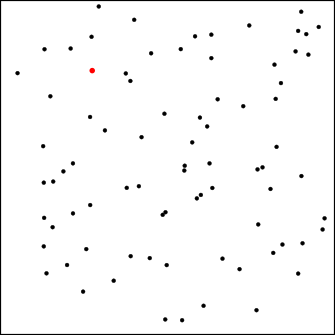
\includegraphics{imgs/treecode-basic}
	\caption{We want to calculate the force on the red dot in this system, which involves 79 calculations (since there are 80 bodies). These 79 calculations must be repeated for every other body, for a total of $79*80=6320$ calculations.}
	\label{treecode-basic}
\end{figure}

\begin{figure}[p]
	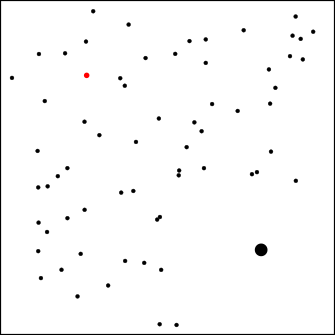
\includegraphics{imgs/treecode-merged}
	\caption{The force on the red body in this system is similar to the one seen earlier. However, the number of calculations has been significantly reduced, because about 10 bodies have been replaced with one large body.}
	\label{treecode-merged}
\end{figure}

Our next task is to find an algorithm to do all these merges and accuracy judgements as quickly as possible. Representing space as a kind of tree structure makes this easy to do. To build this tree, space is divided into nodes along each axis (so a 2-dimensional node will have 4 children, while a 3-dimensional one will have 8). Each of these child nodes is then bisected in the same manner, and the process repeats recursively until each bottom-level node has 0 or 1 bodies in it. The resulting structure is referred to as a quadtree (in 2D space) or an octotree (in 3D space). The first two levels of a quadtree can be seen in figure \ref{treecode-nodelev2}.

\begin{figure}[p]
	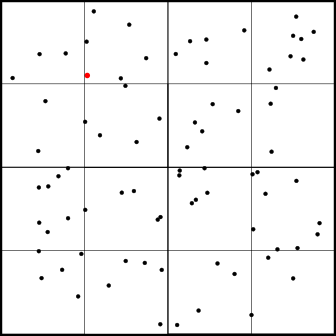
\includegraphics{imgs/treecode-nodelev2}
	\caption{The quadtree after two levels of bisections. Note the 4 child nodes of each node, and the ease of scaling this structure to an arbitrary dimension.}
	\label{treecode-nodelev2}
\end{figure}

Then, to create a system that approximates the original, we simply have to ``walk'' through the tree, deciding whether each node is a suitably accurate approximation for the bodies contained within, or whether its children should be considered individually. This decision is based on the mass of the node and its distance from the body of interest, as well as an ``accuracy factor'' that controls the allowable level of error. Eventually, a list of nodes is created that contains each body exactly once, and the net force can be found by summing up the forces from each node. Figure

\begin{figure}[p]
	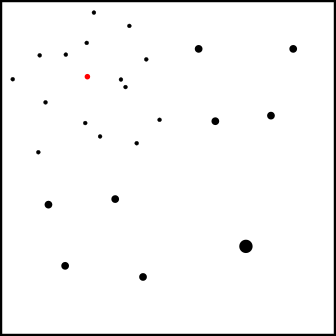
\includegraphics{imgs/treecode-nodes-final}
	\caption{This system is a good approximation of the one considered earlier, and only requires 24 calculations---nearly 75\% less than before. Of course, a real algorithm would be far more rigorous, and likely find even more opportunities to merge bodies.}
	\label{treecode-nodes-final}
\end{figure}

The algorithm discussed here has a time complexity of O$(n \log n)$ in the average case, and O$(n^2)$ in the very worst case. This means that it will practically always beat the na\"ive algorithm for systems of more than a few bodies, and becomes very valuable for large simulations. The creationand analysis of the tree does add some overhead, but a well written implementation will rarely take longer than a few dozen force calculations---while eliminating hundreds or even thousands.



\chapter*{Conclusion}
         \addcontentsline{toc}{chapter}{Conclusion}
	\chaptermark{Conclusion}
	\markboth{Conclusion}{Conclusion}
	\setcounter{chapter}{4}
	\setcounter{section}{0}

\emph{The process by which the structure and dynamics of the MW were discovered was by no means trivial: Linblad [ref.] was a hero along with the other pioneers.  Buried in the galaxy they had some advantages compared to understanding, say, the Andromeda, but being in the disk causes huge difficulties, not the least of which is the dust.}

\section{More info}
And here's some other random info: the first paragraph after a chapter title or section head \emph{shouldn't be} indented, because indents are to tell the reader that you're starting a new paragraph. Since that's obvious after a chapter or section title, proper typesetting doesn't add an indent there.


%If you feel it necessary to include an appendix, it goes here.
\begin{appendices}
    \chapter{}
        \section{The Hubble Classification System} \label{hubble-fork}
            The Hubble Classification System, or Hubble Sequence, is the most commonly used scheme for classifying galaxies. Nicknamed \emph{The Fork}, it goes from elliptical galaxies on the left, to the two kinds (barred and unbarred) of spiral galaxies on the right.

            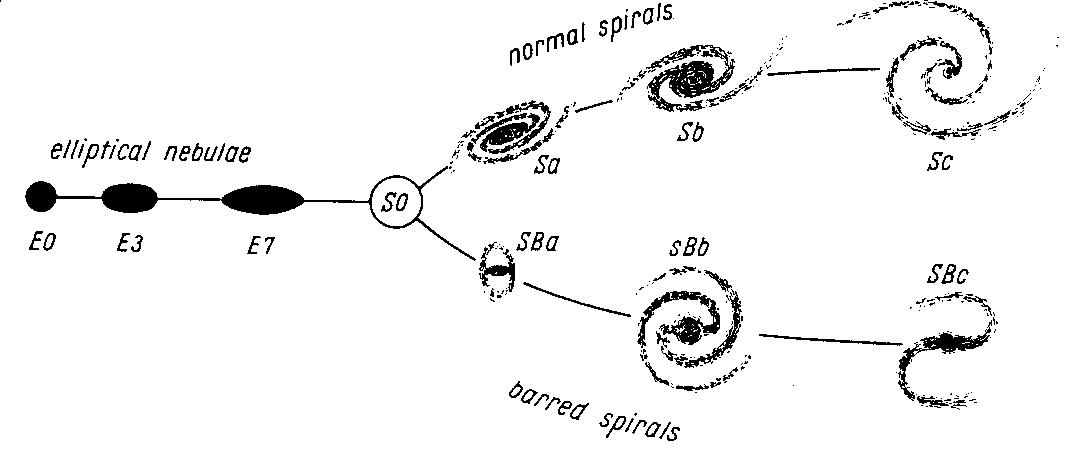
\includegraphics[width=\textwidth]{imgs/hubble_seq}
            \emph{Image courtesy Allan Sandage/CalTech}


        \section{C Language Resources} \label{C-resources}
        \begin{itemize}
            \item \emph{Learn C the Hard Way: Practical Exercises on the Computational Subjects You Keep Avoiding (Like C)}
            ---A good introduction to writing simple, useful C programs. Often breaks with tradition, but always for the better.

            \url{http://www.indiebound.org/book/9780321884923}

            \item \emph{C in a Nutshell}
            ---A massive, 824 page book, that has everything you could ever want to know about using the C language

            \url{http://www.indiebound.org/book/9781491904756}

            \item \emph{21st Century C}
            ---A guide to using a language designed in 1970, in 2017. Most useful if you already have an understanding of C.

            \url{http://www.indiebound.org/book/9781491903896}

            \item \emph{The C Programming Language}
            ---An absolute classic, written by the designers of the language. This book isn't all that useful for \emph{learning} modern C, but it sheds light on the reasons the language was designed the way it was.

            \url{http://www.indiebound.org/book/9780131103627}

            \item \emph{Build your own Lisp}
            ---Learn C by writing an interpreter for the Lisp language. A complete guide to a really fun and useful project. Available both online and as a printed book.

            \url{http://www.buildyourownlisp.com}

            \url{http://www.indiebound.org/book/9781501006623}
        \end{itemize}
\end{appendices}


%This is where endnotes are supposed to go, if you have them.
%I have no idea how endnotes work with LaTeX.

  \backmatter % backmatter makes the index and bibliography appear properly in the t.o.c...

% if you're using bibtex, the next line forces every entry in the bibtex file to be included
% in your bibliography, regardless of whether or not you've cited it in the thesis.
    \nocite{*}

% Rename my bibliography to be called "Works Cited" and not "References" or ``Bibliography''
% \renewcommand{\bibname}{Works Cited}

%    \bibliographystyle{bsts/mla-good} % there are a variety of styles available;
%  \bibliographystyle{plainnat}
% replace ``plainnat'' with the style of choice. You can refer to files in the bsts or APA
% subfolder, e.g.
 \bibliographystyle{APA/apa-good}  % or
 \bibliography{thesis}
 % Comment the above two lines and uncomment the next line to use biblatex-chicago.
 %\printbibliography[heading=bibintoc]

% Finally, an index would go here... but it is also optional.
\end{document}
